%% =====================================================================
%%  AutoDev -- IEEE conference paper (IEEEtran, two-column)
%% ---------------------------------------------------------------------
%%  FORMATTING NOTES (IEEE conference style)
%%   * Class: IEEEtran, [conference] option, US Letter (use a4paper if the
%%     venue asks for A4). Two columns, 0.17in (~4.2 mm) column gap.
%%   * Fonts: Times (via newtxtext/newtxmath) -- the Times New Roman
%%     equivalent IEEE requires. Body 10 pt, title 24 pt, author names
%%     11 pt, affiliations 10 pt italic, abstract/index terms 9 pt bold,
%%     section heads 10 pt small caps (roman numerals), subsection heads
%%     10 pt italic (A., B., ...), captions 8 pt, references 8 pt.
%%   * Single line spacing; no page numbers or headers (the venue adds them).
%%   * Figures/tables: captions ABOVE tables, BELOW figures. Use figure* /
%%     table* only for floats that must span both columns.
%%   * Placeholders still to be filled are typeset in red via \tbd{}.
%%     Search this file for "\tbd" before submission and delete the macro
%%     definition last so any leftover placeholder fails to compile.
%%  Compile: pdflatex -> pdflatex (twice, for cross-references).
%% =====================================================================
\documentclass[conference,letterpaper]{IEEEtran}
\IEEEoverridecommandlockouts

\usepackage[T1]{fontenc}
% Times New Roman equivalent: newtx on Overleaf/full TeX Live, mathptmx fallback
\IfFileExists{newtxtext.sty}{\usepackage{newtxtext,newtxmath}}{\usepackage{mathptmx}}
\usepackage{cite}
\usepackage{amsmath,amsfonts}
\usepackage{graphicx}
\usepackage{booktabs}
\usepackage{multirow}
\usepackage{array}
\usepackage{xcolor}
\usepackage{algorithm}
\usepackage{algpseudocode}
\usepackage{balance}
\usepackage[hidelinks]{hyperref}

\graphicspath{{figs/}}

%% Placeholder marker: red text, easy to find and replace.
\newcommand{\tbd}[1][--]{\textcolor{red}{#1}}
\newcommand{\ph}[1]{\textcolor{red}{[#1]}}

%% Lets the author block break onto a second row (3 + 2 authors).
\makeatletter
\newcommand{\linebreakand}{%
  \end{@IEEEauthorhalign}
  \hfill\mbox{}\par
  \mbox{}\hfill\begin{@IEEEauthorhalign}}
\makeatother

\begin{document}

%% ------------------------------------------------------------- TITLE
\title{AutoDev: A Human-in-the-Loop, Execution-Verified\\
Multi-Agent Framework for Requirement-to-Code\\
Software Generation under LLM Rate Limits}

%% ------------------------------------------------------------ AUTHORS
\author{
\IEEEauthorblockN{Pradyot Bilurkar}
\IEEEauthorblockA{\textit{Dept. of Artificial Intelligence}\\ \textit{and Machine Learning}\\
\textit{B.M.S. College of Engineering}\\
Bengaluru, India\\
USN: 1BM23AI127\\
pradyot.ai23@bmsce.ac.in}
\and
\IEEEauthorblockN{Pranjal Sen}
\IEEEauthorblockA{\textit{Dept. of Artificial Intelligence}\\ \textit{and Machine Learning}\\
\textit{B.M.S. College of Engineering}\\
Bengaluru, India\\
USN: 1BM23AI131\\
pranjalsen.ai23@bmsce.ac.in}
\and
\IEEEauthorblockN{Prem Rathod}
\IEEEauthorblockA{\textit{Dept. of Artificial Intelligence}\\ \textit{and Machine Learning}\\
\textit{B.M.S. College of Engineering}\\
Bengaluru, India\\
USN: 1BM23AI133\\
premRathod.ai23@bmsce.ac.in}
\linebreakand
\IEEEauthorblockN{Rahul Hongekar}
\IEEEauthorblockA{\textit{Dept. of Artificial Intelligence}\\ \textit{and Machine Learning}\\
\textit{B.M.S. College of Engineering}\\
Bengaluru, India\\
USN: 1BM23AI139\\
rahul.ai23@bmsce.ac.in}
\and
\IEEEauthorblockN{Shridevi A. Desai}
\IEEEauthorblockA{\textit{Assistant Professor, Dept. of Artificial Intelligence}\\
\textit{and Machine Learning}\\
\textit{B.M.S. College of Engineering}\\
Bengaluru, India\\
shrideviad.mel@bmsce.ac.in}
}

\maketitle

%% ----------------------------------------------------------- ABSTRACT
\begin{abstract}
Large language models (LLMs) can synthesise code from a natural-language
prompt, but single-prompt generation skips the requirements analysis, design
review and execution-based testing that a software team performs, so the output
often fails to build or drifts from the request. Role-based multi-agent
frameworks restore the missing roles, yet most pass free-form text between
agents, give the human owner no defined point of control, and accept code on
another model's opinion rather than on running it. This paper presents
\emph{AutoDev}, a LangGraph framework in which Product Manager, Architect,
Developer and QA agents exchange only validated Pydantic contracts, a human
approves the requirements and the architecture at two persistent interrupt
gates, and the generated project is compiled, linted and executed against
tests before it is accepted. Failures are attributed to the service that
caused them and returned as real compiler output and tracebacks, so only
failing services are regenerated within a bounded retry budget. A
provider-agnostic LLM layer adds a rolling token budget that learns the
provider's true per-minute limit, a retry/degrade/abort error classifier, a
four-rung structured-output ladder and difficulty-based model routing. On 141
injected faults, verification detected 88.7\%, with the static gate catching
every build fault about $25\times$ faster than test execution; attribution
reached 100\% precision and recall and cut Developer calls by 64.4\%; and
under a simulated 8{,}000 TPM provider the self-correcting budget reduced
rate-limit rejections from 48 to 1. End-to-end results with live models are
reported in Section~VI.
\end{abstract}

\begin{IEEEkeywords}
multi-agent systems, large language models, automated software engineering,
code generation, human-in-the-loop, execution feedback
\end{IEEEkeywords}

%% ======================================================== I. INTRODUCTION
\section{Introduction}

Code-capable LLMs have made it routine to turn a short description into a
working function~\cite{chen2021codex,austin2021mbpp,roziere2023codellama}.
Building an application is a different task. A human team first fixes
\emph{what} is to be built, then \emph{how} it is structured, and only then
writes, reviews and tests the code; each step constrains the next. When a
single prompt replaces this sequence, a misreading of the requirement flows
silently into code that nobody has run.

Role-based multi-agent frameworks such as MetaGPT~\cite{hong2024metagpt} and
ChatDev~\cite{qian2024chatdev} reintroduce the missing roles by assigning LLM
agents to them, and report clear gains over single-agent generation. In
practice, four gaps remain.

\begin{enumerate}
\item \emph{Unchecked hand-offs.} Agents usually exchange free text or loosely
structured documents. A downstream agent can receive an incomplete or malformed
artifact and keep going, so the error surfaces several stages later, far from
its cause.
\item \emph{No defined human control point.} The person who owns the requirement
rarely gets a fixed moment to correct the plan before code is written, which is
when a correction is cheapest.
\item \emph{Opinion instead of execution.} Quality is often judged by another
LLM reading the code. A reviewer model can approve code that does not import.
\item \emph{Operational fragility.} Free-tier and self-hosted deployments add
per-minute token limits and model-specific capability gaps, such as weak tool
calling, that end long multi-agent runs part-way through.
\end{enumerate}

\textbf{Problem statement.} Given a one-paragraph natural-language requirement,
produce a multi-service Python back-end project whose requirements and design
have been approved by a human, whose code has been shown to compile, pass a
linter and pass tests, and do so reliably on affordable, rate-limited LLM
providers.

AutoDev addresses this problem with a single LangGraph~\cite{langgraph} state
graph whose nodes are four role agents, two human review gates, a static gate
and a sandboxed test runner, backed by an LLM layer engineered for rate limits.
Its specific contributions are summarised in Section~IV.

\textbf{Organisation.} Section~II reviews related work. Section~III describes
the architecture and methodology, and Section~IV states the novel
contributions. Section~V covers implementation, Section~VI the evaluation, and
Section~VII concludes with future work.

%% ======================================================== II. RELATED WORK
\section{Related Work}

\subsection{LLMs for Code Generation}
Codex and the HumanEval benchmark~\cite{chen2021codex}, together with
MBPP~\cite{austin2021mbpp}, made functional correctness on held-out unit tests
the standard measure of generated code, reported as pass@$k$. AlphaCode~\cite{li2022alphacode}
showed that sampling many candidates and filtering them by execution scales to
competitive programming, and CodeT~\cite{chen2023codet} used model-generated
tests to rank candidates. SWE-bench~\cite{jimenez2024swebench} moved evaluation
to resolving real repository issues. A systematic review~\cite{hou2024llm4se}
notes that most systems target isolated tasks rather than the full
requirement-to-deployment life cycle.

\subsection{Multi-Agent Software Development}
MetaGPT~\cite{hong2024metagpt} encodes standard operating procedures and has role
agents publish structured documents to a shared message pool.
ChatDev~\cite{qian2024chatdev} arranges agents in a waterfall-style chat chain of
design, coding and testing, and offers an optional mode in which a person plays
the reviewer. AgentCoder~\cite{huang2023agentcoder} separates a
programmer, a test designer and a test executor, and MapCoder~\cite{islam2024mapcoder}
chains retrieval, planning, coding and debugging agents.
AutoGen~\cite{wu2023autogen} provides a general conversation framework for
composing agents, and OpenHands~\cite{wang2025openhands} offers an open platform
for agents that act in a sandboxed development environment. These systems
establish the value of role decomposition but typically treat the inter-agent
protocol, human oversight and resource limits as secondary concerns.

\subsection{Execution Feedback and Self-Repair}
Self-Debugging~\cite{chen2024selfdebug}, Self-Refine~\cite{madaan2023selfrefine}
and Reflexion~\cite{shinn2023reflexion} show that feeding execution results or
verbal feedback back to the model improves correctness.
SWE-agent~\cite{yang2024sweagent} demonstrates the value of a purpose-built
agent--computer interface, and Agentless~\cite{xia2024agentless} shows that a
fixed localise--repair--validate pipeline can rival free-form agents.
ReAct~\cite{yao2023react} interleaves reasoning with tool actions.

\subsection{Gap Addressed}
Table~\ref{tab:related} contrasts AutoDev with representative systems. To our
knowledge, none of them combines schema-validated hand-offs that fail closed,
persistent human approval gates, project-level execution feedback with
per-service attribution, and an LLM layer designed for rate-limited providers.

\begin{table}[t]
\caption{Comparison with Representative Systems}
\label{tab:related}
\centering
\footnotesize
\setlength{\tabcolsep}{3pt}
\resizebox{\columnwidth}{!}{%
\begin{tabular}{@{}lccccc@{}}
\toprule
Capability & MetaGPT & ChatDev & AgentCoder & SWE-agent & AutoDev \\
\midrule
Role decomposition      & \checkmark & \checkmark & \checkmark & -- & \checkmark \\
Schema-validated hand-off & partial & -- & -- & -- & \checkmark \\
Human approval gates    & -- & partial & -- & -- & \checkmark \\
Executes generated tests& partial & partial & \checkmark & \checkmark & \checkmark \\
Per-service attribution & -- & -- & -- & -- & \checkmark \\
Rate-limit-aware budget & -- & -- & -- & -- & \checkmark \\
\bottomrule
\end{tabular}}
\vspace{2pt}

\raggedright\scriptsize Entries reflect the cited papers and public repositories
as read in November 2026. ``Partial'': MetaGPT publishes structured documents and
runs an executable-feedback loop but does not halt on invalid ones; ChatDev's
testing phase uses compiler feedback, and its optional Human-Agent-Interaction mode
lets a person act as reviewer but has no fixed approval points; SWE-agent enforces
a per-run cost limit, which is not a token-rate budget.
\end{table}

%% ============================================ III. METHODOLOGY / ARCHITECTURE
\section{Methodology and System Architecture}

\subsection{Layered Architecture}
AutoDev is organised in six layers (Fig.~\ref{fig:arch}). A command-line client
and a Next.js console are both clients of one FastAPI service, so a run started
in one is visible in the other. The service persists runs in SQLite, streams
progress over Server-Sent Events (SSE) and packages results as a zip archive.
Orchestration is a LangGraph \texttt{StateGraph} over a shared state object; a
SQLite-backed checkpointer lets a run paused for human review survive a server
restart. Agents never call a model directly: every call passes through the LLM
layer, which selects the provider and model, enforces the token budget and
extracts structured output.

\begin{figure}[t]
\centering
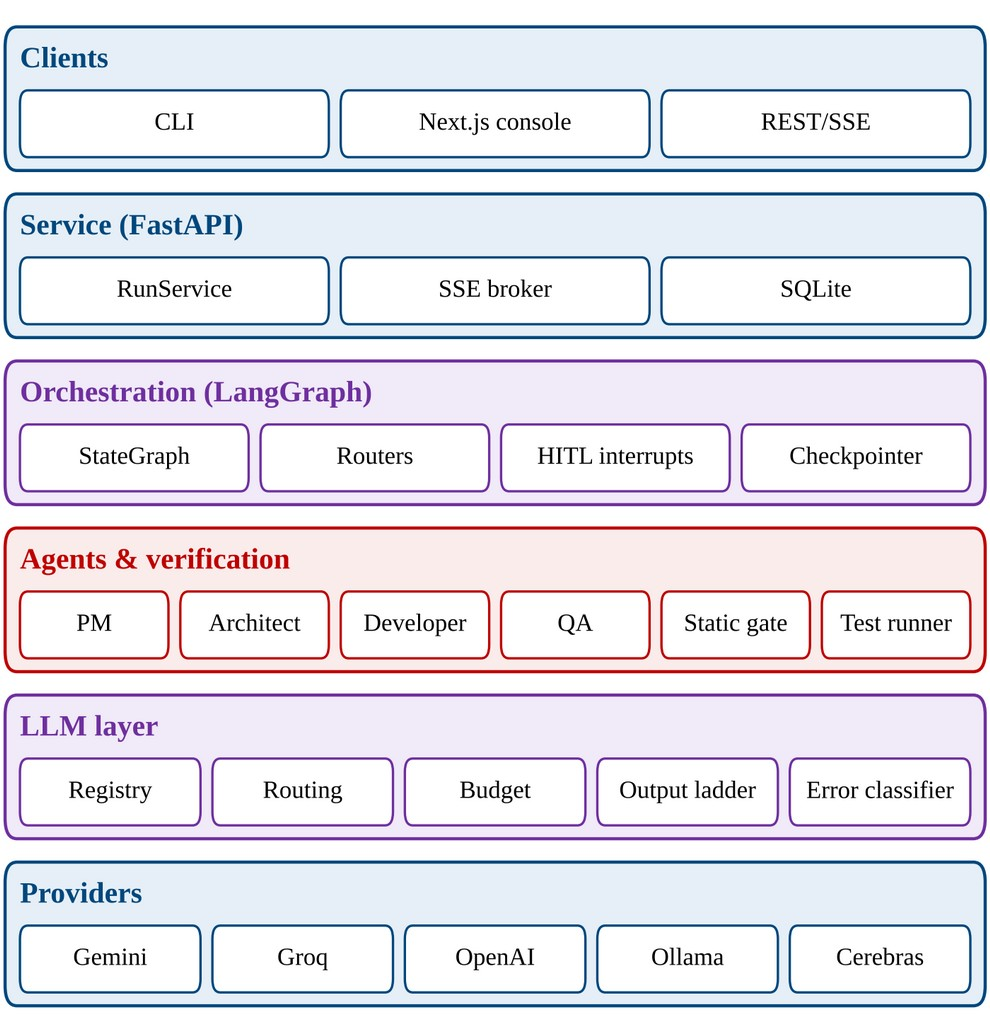
\includegraphics[width=0.86\columnwidth]{fig1_architecture.png}
\caption{Layered architecture of AutoDev. Every model call from the agent layer
passes through the LLM layer.}
\label{fig:arch}
\end{figure}

Each run receives an isolated workspace holding the JSON (and optional PDF)
artifact of every stage, the generated source and tests, the final archive and
the full log. Every file path in a generated manifest is resolved against this
workspace and rejected if it would escape it.

\subsection{Typed Agent Contracts}
Table~\ref{tab:agents} lists the agents, what each reads from the shared state
and the contract it must satisfy. The PM agent turns the requirement into a
product requirements document (PRD) with prioritised features, data entities,
endpoints, user flows and non-functional requirements. The Architect produces
services, endpoints, data models, databases, environment variables and
implementation tasks. The Developer writes per-service source files, and QA
returns bugs with severities, per-service quality scores and test files. Each
agent has two prompts: a structured prompt for the JSON contract consumed by the
next agent, and a text prompt for an optional client-facing PDF (off by default,
since the console renders the same documents from the JSON).

\begin{table}[t]
\caption{Agents and Their Contracts}
\label{tab:agents}
\centering
\footnotesize
\begin{tabular}{@{}l>{\raggedright}p{2.6cm}>{\raggedright\arraybackslash}p{2.95cm}@{}}
\toprule
Agent & Reads & Writes (contract) \\
\midrule
PM        & requirement, PM feedback & PRD\newline(\texttt{ManagerSchema}) \\
Architect & PRD, architect feedback  & architecture\newline(\texttt{ArchitectSchema}) \\
Developer & PRD projection, architecture, failure evidence & code manifest\newline(\texttt{DeveloperSchema}) \\
QA        & manifest, selected source files & report + tests\newline(\texttt{QASchema}) \\
\bottomrule
\end{tabular}
\end{table}

Agents see \emph{projections} of earlier artifacts rather than whole documents:
the Developer, for example, works from the architecture and receives only the
PRD fields it needs. In one observed run the full PRD alone was 3{,}057 tokens
against an 8{,}000 token-per-minute (TPM) limit, so narrowing the prompt copy,
while leaving the stored artifact unchanged, directly reduces rate-limit
pressure.

\subsection{Pipeline Graph and Human Review}
Fig.~\ref{fig:pipeline} shows the graph. LangGraph interrupts after the PM and
Architect nodes. An empty response approves the artifact; non-empty feedback is
written to the state and routes the graph back to the same agent, which revises
its \emph{previous} output rather than starting over. Every edge leaving a node
is conditional: if the node's status is \emph{failed}, the router ends the run,
because every downstream agent depends on the artifact that was not produced.
Continuing would spend tokens writing code against an empty architecture and
bury the real error under whatever broke next.

\begin{figure}[t]
\centering
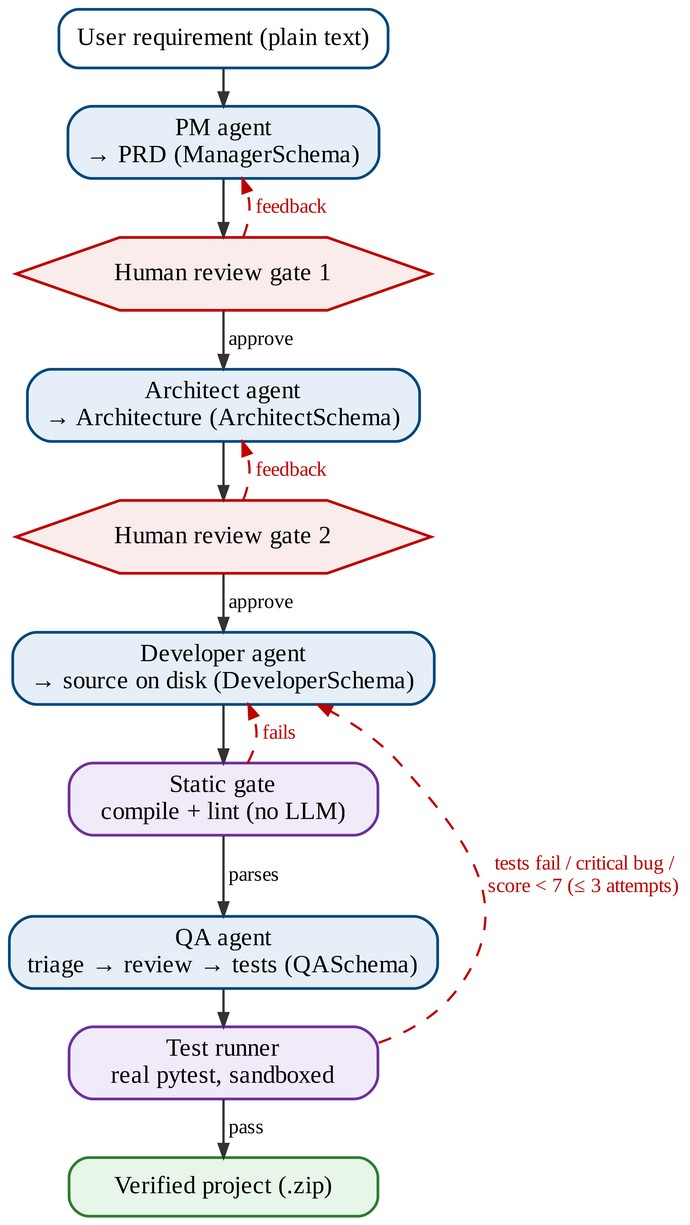
\includegraphics[width=0.62\columnwidth]{fig2_pipeline.png}
\caption{Agent pipeline. Solid edges are the forward path; dashed red edges are
human revision loops and verification-driven repair loops.}
\label{fig:pipeline}
\end{figure}

\subsection{Execution-Based Verification and Repair}
\label{sec:verification}
Verification is ordered by cost (Algorithm~\ref{alg:verify}). The static gate
compiles every generated Python file and runs the Ruff linter per service, with
no model call; code that does not parse goes straight back to the Developer. It
also checks what a compiler and a linter cannot see but live runs kept
producing: an import of a name or module that no file of the service defines, a
module hidden by a same-named package (Python imports the package), and APIs a
library has moved, such as \texttt{BaseSettings} leaving Pydantic~2 for
\texttt{pydantic-settings}. Before anything is written, generated files whose
line breaks arrive escaped as literal \texttt{\textbackslash n} are restored when
the restored text parses.
Code that parses reaches QA, which reviews in two steps: a cheap triage call
sees only the file manifest and selects the files worth reading, and only those
files are loaded and scored. The test runner then installs the project's
dependencies and executes the pytest files QA wrote, together with one test it
adds itself: that the application imports. Without it, a QA suite that only
exercises schemas can pass while the application cannot start, and an import
failure is reported with the project file and line that caused it.

Let $T$ be the number of failing or erroring tests, $K$ the number of services
whose tests could not run, $C$ the number of critical bugs and $s_i$ the quality
score of service $i$. The graph returns to the Developer when
\begin{equation}
(T>0)\;\lor\;(K>0)\;\lor\;(C>0)\;\lor\;\bigl(\min_i s_i<\tau\bigr)
\label{eq:retry}
\end{equation}
and the attempt counter $a$ is below its limit $A$, with $\tau=7$ and $A=3$ by
default. Real test failures are checked before the reviewer's opinion.

\begin{algorithm}[t]
\caption{Cost-ordered verification and surgical repair}
\label{alg:verify}
\small
\begin{algorithmic}[1]
\Require architecture $\mathcal{A}$, services $S$, limit $A$
\State $a \gets 0$;\; $R \gets S$ \Comment{services to (re)generate}
\Loop
  \State generate code for each $s\in R$ using its evidence $E_s$
  \State $a \gets a+1$
  \State $F \gets \textsc{StaticGate}(S)$ \Comment{compile + lint, no LLM}
  \If{$F\neq\emptyset$}
     \State $E \gets F$
  \Else
     \State $Q \gets \textsc{QA}(\textsc{Triage}(\text{manifest}))$
     \State $T \gets \textsc{RunTests}(Q.\text{tests})$ \Comment{sandboxed}
     \If{Eq.~(\ref{eq:retry}) is false} \Return \textsc{Pass}
     \EndIf
     \State $E \gets T \cup Q.\text{bugs}$
  \EndIf
  \If{$a \ge A$} \Return \textsc{Fail} \EndIf
  \State $R \gets \textsc{Attribute}(E)$;\; $E_s \gets \{e\in E : \text{svc}(e)=s\}$
\EndLoop
\end{algorithmic}
\end{algorithm}

\textbf{Failure attribution.} Static failures carry the slug of the service they
ran over, test results name their service, and QA bugs name a file that the code
manifest maps to a service. Each service is then shown only its own failures,
and only implicated services are regenerated; the rest are kept byte-for-byte.
A project with four services and one failure therefore costs one model call
instead of four.

\textbf{Service identity.} Attribution and surgical regeneration both key on a
service's name, so the Developer is instructed to spell each service exactly as
the architecture does. The instruction alone did not hold: in a live run, a
preview model asked for ``Bookmark API Service'' returned complete code under
``bookmark\_api'', and the whole answer was discarded as off-target. Because the
Developer is called once per service, a response that contains exactly one
service is now assigned the requested name, unless that name belongs to a
\emph{different} service of the same project, in which case the response is
still rejected rather than written into the wrong service's directory. Service
identity is therefore enforced by the orchestrator, not delegated to the model.

\subsection{Rate-Limit-Aware LLM Layer}
\textbf{Token budget.} Providers meter tokens over a rolling minute, and they
charge the requested completion ceiling, not the tokens actually produced.
Before each call the budget reserves
\begin{equation}
r=\hat{p}+c
\label{eq:reserve}
\end{equation}
where $\hat{p}$ is the estimated prompt size and $c$ the completion ceiling, and
admits the call only if
\begin{equation}
\sum_{t\in(\text{now}-60\,\text{s},\,\text{now}]} u(t)\;+\;r\;\le\;L
\label{eq:window}
\end{equation}
where $u(t)$ are the reserved or reconciled usages in the window and $L$ is the
ceiling; otherwise it waits. After the call the reservation is reconciled with
the reported usage. A rolling rather than fixed window avoids admitting twice
the limit across a minute boundary. The budget is keyed by provider account and
model, not by agent, because the quota belongs to the account. When a 429
response states the real limit and current usage, both are adopted; in one run
the configured 12{,}000 TPM was corrected to the enforced 8{,}000. A single call
larger than $L$ raises an error instead of waiting forever.

\textbf{Error disposition.} Each failure is classified from its status code or
message into one of three outcomes (Table~\ref{tab:errors}). Unrecognised errors
degrade rather than retry, since repeating a deterministic failure only consumes
budget needed by later agents.

\begin{table}[t]
\caption{Error Disposition}
\label{tab:errors}
\centering
\footnotesize
\begin{tabular}{@{}l>{\raggedright}p{3.0cm}>{\raggedright\arraybackslash}p{2.6cm}@{}}
\toprule
Disposition & Examples & Action \\
\midrule
Retry   & 429, 5xx, timeout, dropped connection & same call after provider-advised or exponential wait \\
Degrade & 400 tool-call or schema error, validation error & next strategy or provider, no repeat \\
Abort   & invalid key, retired model, call $>$ budget & stop the run \\
\bottomrule
\end{tabular}
\end{table}

\textbf{Structured-output ladder.} Agents request a schema, never a mechanism.
For each model the layer builds a ladder of extraction strategies, skipping rungs
the provider cannot support (Table~\ref{tab:ladder}). Because the last rung needs
only plain text, any chat model can drive the pipeline. For example, a small
Groq-hosted Llama model returned its JSON wrapped in a pseudo function-call tag,
which the provider rejected as a tool-use failure; the parse rung recovered the
object.

\begin{table}[t]
\caption{Structured-Output Ladder}
\label{tab:ladder}
\centering
\footnotesize
\begin{tabular}{@{}ll@{}}
\toprule
Rung & How the schema is enforced \\
\midrule
\texttt{native}      & provider default, normally tool calling \\
\texttt{json\_schema}& constrained decoding to the schema \\
\texttt{json\_mode}  & valid JSON guaranteed; schema in prompt \\
\texttt{parse}       & plain text; locate and validate JSON \\
\bottomrule
\end{tabular}
\end{table}

\textbf{Difficulty routing and escalation.} Models are configured per
\emph{purpose} (heavy code generation, structured documents, PDF text, cheap
triage) rather than per agent. For code generation, each service receives a
deterministic difficulty score computed from the architecture,
\begin{equation}
d = 2F + E + M + 2D
\label{eq:difficulty}
\end{equation}
where $F$, $E$, $M$ and $D$ are its key files, endpoints, data models and service
dependencies. Services with $d<12$ use the low tier, $d\ge48$ the high tier,
and the rest the medium tier. Routing is off by default, and the experiments in
Section~VI use a single model for every purpose, so they do not exercise it. If verification shows that a tier was too weak, the
service is escalated by at most one tier, and never for failures a stronger model
cannot fix, such as rate limits or rejected keys. Completion ceilings are likewise
sized per purpose and narrowed when the expected answer size is known.

\subsection{Sandboxed Execution}
Generated code is treated as untrusted. The runner executes it with a scrubbed
environment containing no API keys, a working directory pinned inside the run
workspace, a wall-clock timeout and a cap on captured output. A runner protocol
allows a container backend to replace the local subprocess runner.

%% =============================================== IV. NOVELTY & CONTRIBUTIONS
\section{Novelty and Contributions}

Compared with the baselines in Section~II, AutoDev makes six distinct
contributions.

\textbf{N1. Contract-first, fail-closed orchestration with persistent human
gates.} Every hand-off is a validated Pydantic schema, every edge is conditional
on the producing node's status, and the two human review gates are graph
interrupts backed by a durable checkpointer. A malformed artifact can therefore
never reach the next agent, and a run waiting for approval survives a restart.
Prior frameworks either exchange free text~\cite{qian2024chatdev} or publish
structured documents without halting on invalid ones~\cite{hong2024metagpt}, and
none places the requirement owner at fixed, resumable control points.

\textbf{N2. Cost-ordered, execution-verified repair with per-service failure
attribution.} Verification runs in increasing order of cost (a model-free static
gate, a two-step QA review, then sandboxed tests), and real tracebacks outrank a
reviewer's score. Each failure is traced to the service that produced it, so only
implicated services are regenerated and each sees only its own evidence. This
moves execution feedback~\cite{chen2024selfdebug,shinn2023reflexion} from single
functions to multi-service projects and makes the repair cost proportional to the
number of failing services rather than to project size.

\textbf{N3. A self-correcting, account-scoped token budget with a three-way error
disposition.} The budget reserves prompt plus completion ceiling over a rolling
window, is shared by all agents on one account, and learns the enforced limit from
the provider's first 429 response. Combined with a classifier that retries only
transient errors, this treats provider quotas as a first-class constraint of
multi-agent design rather than an operational afterthought.

\textbf{N4. Capability-agnostic structured output and deterministic difficulty
routing.} A four-rung ladder lets any chat model, including small open-weight
models with unreliable tool calling, satisfy the same contracts, while an
explainable integer difficulty score routes each service to a model tier and
escalates at most one step on evidence. Together these let the pipeline run on
free-tier and local models, not only on frontier APIs.

\textbf{N5. Model-free defences against LLM-specific code defects.} Live runs
produced defects that compile, lint clean and are invisible to a reviewer model:
imports of functions no file defines, a package created beside a same-named module
(which Python then imports instead), library APIs from an older major version, and
whole files whose line breaks arrived escaped. Each is caught or repaired by a
deterministic check that resolves imports the way the interpreter does, before any
model is asked to review the code. The test runner also owns one test that no
agent writes---that the application imports---so a reviewer-written suite cannot
pass ``hollowly'' while the application fails to start; in one observed run, two
schema-only tests passed against an application that crashed on import. The
failure names the project file and line to fix, which is the evidence the next
Developer pass receives.

\textbf{N6. Budget-fitted repair and measured cost.} A repair prompt carries real
compiler output and tracebacks, which can exceed a small per-minute window on
their own. Failure evidence is therefore condensed in graded levels (deduplicated
assertion lines, then fewer failures, then shorter messages) until the whole call,
prompt plus completion ceiling, fits the window, instead of failing the stage. All
model calls are recorded in one ledger at the single point every call passes
through, with the provider's own token counts captured by a callback even when a
structured-output parser discards the raw message, and priced only from published
rates. Cost per verified project is thus measured rather than estimated, and the
same per-service independence that enables attribution lets a project's services
be generated concurrently under the shared budget.

%% =================================================== V. IMPLEMENTATION
\section{Implementation Details}

\subsection{Technology Stack}
Table~\ref{tab:stack} summarises the stack. The back end is Python, with
LangGraph~1.0 for orchestration, Pydantic~v2 for contracts and settings, FastAPI
with SSE for the service, aiosqlite for persistence and fpdf2 for optional
client documents; retries use the error classifier of Section~III-E rather than a
retry library. Gemini~2.5 Flash is the default model; Groq, Ollama, Cerebras and
any OpenAI-compatible API (OpenAI, DeepSeek, Qwen, OpenRouter) are selectable
through LangChain provider packages. The live experiments in Section~VI use
DeepSeek~V4.1 Flash. The console is written in Next.js~14 and TypeScript. Development used VS Code, Git
and GitHub~\cite{autodevrepo}.

\begin{table}[t]
\caption{Technology Stack}
\label{tab:stack}
\centering
\footnotesize
\begin{tabular}{@{}l>{\raggedright\arraybackslash}p{5.1cm}@{}}
\toprule
Layer & Tools \\
\midrule
Orchestration & LangGraph 1.0, SQLite checkpointer \\
Contracts     & Pydantic v2, pydantic-settings \\
LLM providers & Gemini 2.5 Flash (default), Groq, Ollama, Cerebras, OpenAI-compatible APIs (DeepSeek in Sec.~VI) via LangChain \\
Service       & FastAPI, Uvicorn, SSE, aiosqlite \\
Verification  & \texttt{py\_compile}, Ruff, pytest, subprocess sandbox \\
Front end     & Next.js 14, TypeScript \\
Artifacts     & fpdf2 (PDF), zip archive \\
Testing       & pytest (1{,}267 tests), fake LLM for offline runs \\
\bottomrule
\end{tabular}
\end{table}

\subsection{Code Organisation}
The \texttt{agents}, \texttt{llm}, \texttt{verification}, \texttt{graph},
\texttt{server}, \texttt{core} and \texttt{schema} packages comprise about
9{,}800 lines of Python, and the console about 7{,}200 lines of TypeScript. All
settings (provider, per-purpose models and completion ceilings, TPM limit, retry
limits, $\tau$ and $A$) are read from environment variables through a single
settings object.

\subsection{Implementation Steps}
\begin{enumerate}
\item \emph{Contracts first.} Pydantic schemas for the PRD, architecture, code
manifest, QA report and verification reports were defined before any agent, so
prompts are written against a fixed target.
\item \emph{Agents and prompts.} Each agent was implemented as a graph node with a
structured prompt and a PDF prompt, reading only a projection of earlier state.
\item \emph{Graph and gates.} Nodes, conditional routers and the two interrupts
were wired in one \texttt{StateGraph}, with checkpointing for resumable runs.
\item \emph{Verification.} The static gate, test runner and sandboxed runner were
added, followed by the attribution module and surgical regeneration.
\item \emph{LLM layer.} The provider registry, token budget, error classifier,
structured-output ladder and difficulty router were built and unit-tested with a
fake LLM and a simulated clock.
\item \emph{Service and console.} A FastAPI service with fifteen routes (health;
create, list, read, delete, approve, give feedback to and cancel runs; read the log
and stream events; list and read files and artifacts, export a document as PDF,
and download the archive) and the Next.js console were built on top of the same run service.
\end{enumerate}

\begin{figure}[t]
\centering
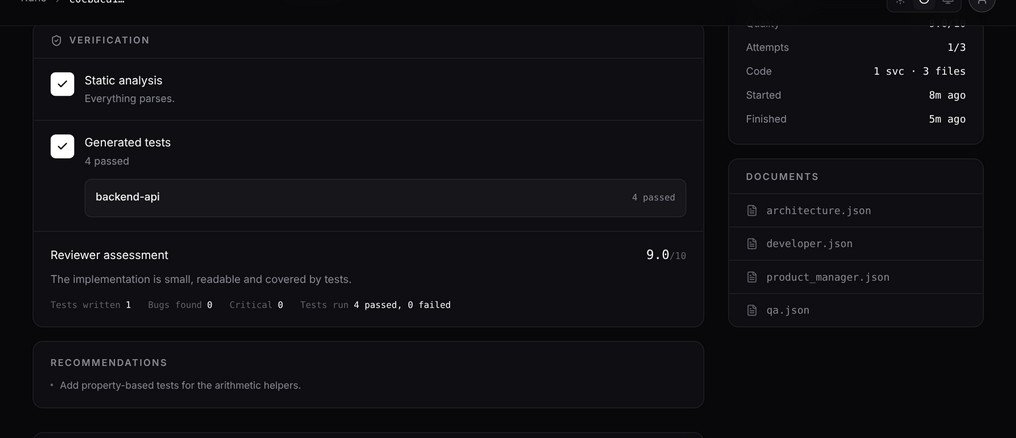
\includegraphics[width=\columnwidth]{fig3_console.png}
\caption{Console view of a completed run: static analysis and generated-test
results, reviewer score and stored artifacts.}
\label{fig:console}
\end{figure}

The console (Fig.~\ref{fig:console}) shows the stage stepper, the review panel,
the PRD and architecture, verification results, the file tree and the live log.

%% ============================================ VI. RESULTS, EVALUATION, DISCUSSION
\section{Results, Evaluation and Discussion}

\subsection{Evaluation Design and Research Questions}
We evaluate AutoDev at two levels. \emph{Component-level} experiments exercise
the real code of each mechanism with controlled inputs and are complete.
\emph{System-level} experiments run the full pipeline with live models and are in
progress; their tables below contain placeholders (\tbd[red]) to be filled. The
study answers five research questions:
\begin{itemize}
\item \textbf{RQ1} Does cost-ordered verification detect faults in generated code?
\item \textbf{RQ2} Is failure attribution accurate, and how much does surgical
regeneration save?
\item \textbf{RQ3} Do the ladder, classifier and token budget keep runs alive on
weak, rate-limited providers?
\item \textbf{RQ4} How often does the full pipeline turn a requirement into a
verified project with live models, and at what cost?
\item \textbf{RQ5} How does AutoDev compare with baselines, and what does each
component contribute?
\end{itemize}

Component experiments use four dependency-free reference services (expense
tracker, inventory, authentication, notification worker; 24 tests in total)
written in exactly the layout the Developer agent emits, so the static gate and
test runner process them as generated code. All use a fixed seed (42) and are
reproduced by \texttt{evaluation/\allowbreak component/\allowbreak run\_component\_eval.py}
(RQ1, RQ2) and \texttt{evaluation/\allowbreak component/\allowbreak run\_robustness\_eval.py} (RQ3).

\subsection{Metrics}
Table~\ref{tab:metrics} defines the metrics. Because the output is executable
code, functional metrics (pass rates, pass@$k$) are primary; text-overlap metrics
such as BLEU are not used, since they correlate poorly with correctness for
code~\cite{chen2021codex}. For a problem with $n$ samples of which $c$ pass,
\begin{equation}
\text{pass@}k=\mathbb{E}\Bigl[1-\binom{n-c}{k}\Big/\binom{n}{k}\Bigr].
\label{eq:passk}
\end{equation}

\begin{table}[t]
\caption{Evaluation Metrics}
\label{tab:metrics}
\centering
\footnotesize
\begin{tabular}{@{}>{\raggedright}p{2.3cm}>{\raggedright\arraybackslash}p{5.6cm}@{}}
\toprule
Metric & Definition \\
\midrule
Fault detection rate & detected mutants / injected mutants \\
Attribution P / R / F1 & over implicated vs.\ faulty services \\
Run success rate (RSR) & runs ending with Eq.~(\ref{eq:retry}) false / runs \\
First-attempt success & runs passing with $a=1$ / runs \\
Static / test pass rate & services passing the gate; tests passing \\
QA score & mean of $\min_i s_i$ over successful runs (0--10) \\
Dev.\ attempts & mean $a$ per run \\
Cost & LLM calls and tokens per run \\
Latency & wall-clock time per run, excluding human wait \\
HTTP 429s & rate-limit rejections per run \\
pass@1 & Eq.~(\ref{eq:passk}) on HumanEval / MBPP \\
\bottomrule
\end{tabular}
\end{table}

\subsection{RQ1: Fault Detection by the Verification Layer}
Seven mutation operators~\cite{jia2011mutation} were applied at randomly sampled
sites (at most eight per operator per service): four build faults (syntax error,
undefined name, missing import, invalid JSON) and three logic faults
(arithmetic-operator swap, comparison-operator swap, replacing a returned value
with \texttt{None}). Each of the 141 mutants (75 build, 66 logic) was passed
through the real static gate and test runner (Fig.~\ref{fig:faults}). The static
gate caught 100\% of the build faults and, as expected, none of the logic
faults; the generated tests caught 75.8\% of the logic faults (50 of 66).
Combined, verification detected 88.7\% of injected faults (125 of 141). Ten of
the 16 misses were comparison swaps (such as \texttt{<} to \texttt{<=}) at
boundaries the six tests per service do not exercise, five were replaced return
values and one an arithmetic swap. No clean service was flagged (0 false
positives).

\begin{figure}[t]
\centering
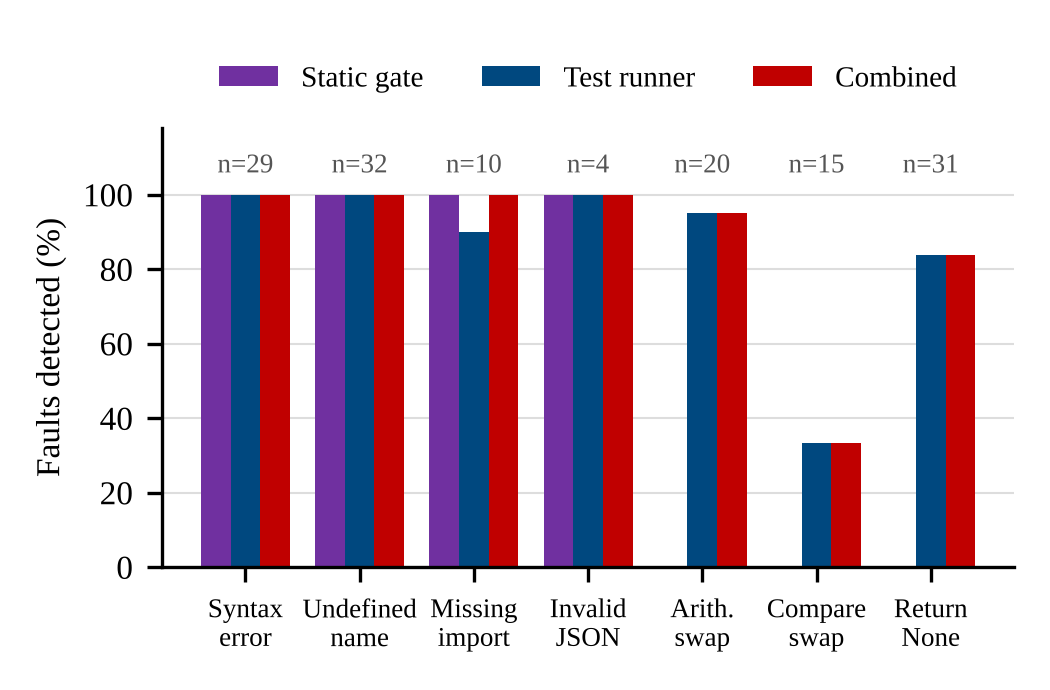
\includegraphics[width=\columnwidth]{fig4_fault_detection.png}
\caption{Share of injected faults detected by the static gate, the test runner
and both combined, per mutation operator ($n$ = mutants).}
\label{fig:faults}
\end{figure}

The ordering of checks pays off: the static gate took a median of 28\,ms per
service against 0.68\,s for the test run, about $25\times$ cheaper, and 60\% of
detected faults (75 of 125) were stopped there, before any QA model call would
have been made. Timings are from a Linux container and will differ by machine.

\subsection{RQ2: Attribution and Surgical Regeneration}
In 40 trials, one to three of the four services were mutated simultaneously and
the whole workspace was verified as the graph does it (static gate first; tests
only if it passes). The services implicated by the attribution module were
compared with the services whose faults were observed. Attribution achieved 100\%
precision and 100\% recall (F1 = 1.0) with an exact set match in every trial.
Regenerating only implicated services needed 57 Developer calls instead of 160
for full regeneration, a 64.4\% reduction.

\subsection{RQ3: Robustness on Weak and Rate-Limited Providers}
\textbf{Structured output.} A valid QA report was rendered in eight output shapes
observed from weaker models (pretty-printed, fenced in markdown, preceded by
prose, followed by prose, surrounded by prose, fenced and surrounded by prose,
wrapped in a pseudo function-call tag, or returned as provider content blocks)
and three unrecoverable shapes (truncated JSON, a missing required field, no
JSON). The parse rung recovered 8/8 recoverable replies against 1/8 for plain
\texttt{json.loads}, and rejected all three invalid ones.

\textbf{Error disposition.} Sixteen provider failures (rate limits, 5xx,
timeouts, tool-call and schema errors, invalid keys, retired models, oversized
requests) were classified with 100\% agreement with Table~\ref{tab:errors}, and
the stated limit, usage and request size were parsed from the Groq 429 message. A
retry-everything policy with three retries would have spent 27 calls on the nine
non-retryable cases.

\textbf{Token budget.} A simulated provider enforced a rolling 8{,}000 TPM window,
charging prompt plus completion ceiling, on a workload of 21 sequential calls
(three pipeline runs of seven calls; 2{,}404--7{,}438 reserved tokens, 6\,s
latency, exponential backoff of 10/20/40\,s without a budget). The real
\texttt{TokenBudget} class was driven with a simulated clock. Without a budget
the workload drew 48 rejections and took 20.8\,min. A static budget configured
with the wrong limit (12{,}000) reduced this to 16 rejections and 16.8\,min.
AutoDev's budget, configured with the same wrong limit but adopting the limit
and usage stated in the first 429, incurred one rejection and finished in
16.3\,min, within about 6\,s of an oracle budget that knew the true limit and
incurred none (Fig.~\ref{fig:ratelimit}).

\begin{figure}[t]
\centering
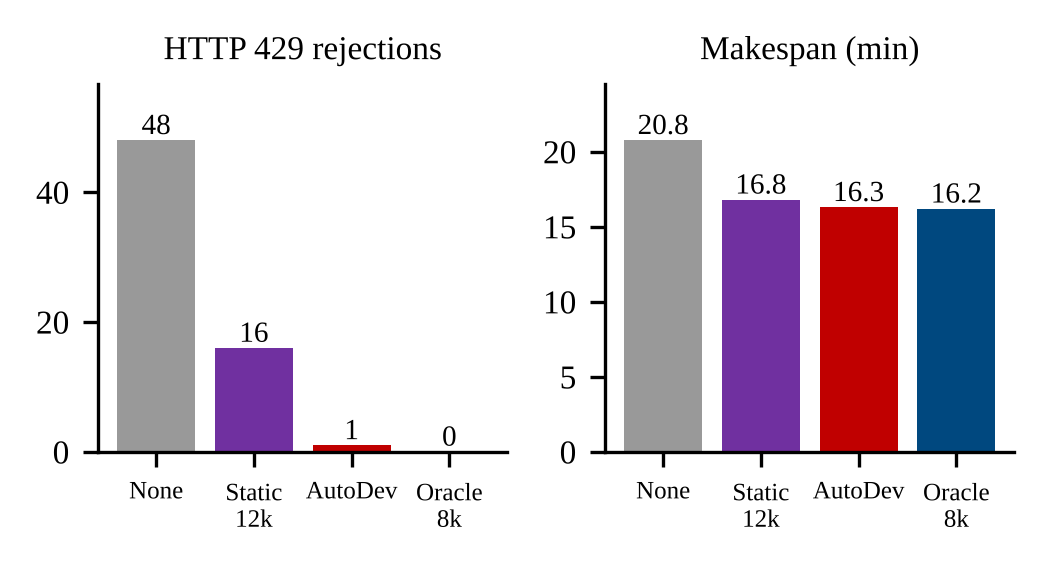
\includegraphics[width=\columnwidth]{fig5_rate_limit.png}
\caption{Rate-limit simulation: HTTP 429 rejections and makespan for no budget,
a static (wrong) budget, AutoDev's self-correcting budget and an oracle.}
\label{fig:ratelimit}
\end{figure}

Table~\ref{tab:component} summarises the component-level results.

\begin{table}[t]
\caption{Component-Level Results}
\label{tab:component}
\centering
\footnotesize
\begin{tabular}{@{}lr@{}}
\toprule
Metric & Result \\
\midrule
Faults detected (all / build / logic) & 88.7\% / 100\% / 75.8\% \\
Static gate vs.\ test run (median)    & 28\,ms vs.\ 0.68\,s \\
Detected faults stopped before QA     & 60\% \\
Attribution precision / recall        & 100\% / 100\% \\
Developer calls saved (surgical)      & 64.4\% \\
Malformed replies recovered           & 8/8 (\texttt{json.loads}: 1/8) \\
Error-disposition accuracy            & 100\% (16 cases) \\
HTTP 429s, no budget vs.\ AutoDev     & 48 vs.\ 1 \\
\bottomrule
\end{tabular}
\end{table}

\textbf{Test suite and offline end-to-end run.} All 1{,}139 automated tests
across 29 modules passed in 262.7\,s; Fig.~\ref{fig:tests} shows their
distribution, with 463 in the LLM layer. In an offline end-to-end run of the
requirement \emph{``Build an expense tracker with login, expense CRUD, and
monthly reports''}, driven by the repository's fake LLM, the pipeline paused at
both review gates, generated a three-file service, passed the static gate, ran
4/4 generated tests and finished on the first attempt with a reviewer score of
9.0/10. With broken code injected, it looped without a QA call and ended as
failed once the retry budget was spent.

\begin{figure}[t]
\centering
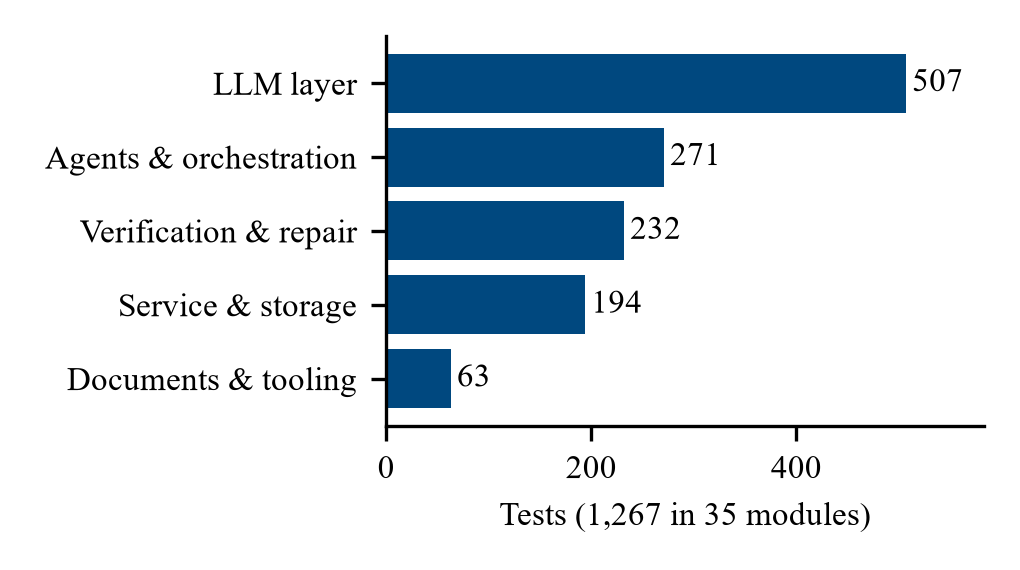
\includegraphics[width=\columnwidth]{fig6_test_distribution.png}
\caption{Distribution of the 1{,}139 automated tests by subsystem.}
\label{fig:tests}
\end{figure}

\subsection{RQ4: End-to-End Benchmark with Live Models}
A benchmark harness (\texttt{evaluation/\allowbreak run\_e2e\_benchmark.py}) runs ten
requirements in three difficulty tiers (\ph{3 easy, 4 medium, 3 hard}), three
times each, through the same service the console uses, with both review gates
auto-approved. Table~\ref{tab:e2e} reports the results per tier and model.

\begin{table*}[t]
\caption{End-to-End Benchmark with Live Models (10 requirements $\times$ 3 runs; mean over runs)}
\label{tab:e2e}
\centering
\footnotesize
\resizebox{\textwidth}{!}{%
\begin{tabular}{@{}llccccccccc@{}}
\toprule
Model & Tier & RSR (\%) & 1st-attempt (\%) & Dev.\ attempts & Static pass (\%) & Test pass (\%) & QA score & LLM calls & Tokens (k) & Latency (min) \\
\midrule
\multirow{4}{*}{Gemini 2.5 Flash}
 & Easy   & \tbd & \tbd & \tbd & \tbd & \tbd & \tbd & \tbd & \tbd & \tbd \\
 & Medium & \tbd & \tbd & \tbd & \tbd & \tbd & \tbd & \tbd & \tbd & \tbd \\
 & Hard   & \tbd & \tbd & \tbd & \tbd & \tbd & \tbd & \tbd & \tbd & \tbd \\
 & \textbf{All} & \tbd & \tbd & \tbd & \tbd & \tbd & \tbd & \tbd & \tbd & \tbd \\
\midrule
\multirow{4}{*}{\ph{Llama (Groq)}}
 & Easy   & \tbd & \tbd & \tbd & \tbd & \tbd & \tbd & \tbd & \tbd & \tbd \\
 & Medium & \tbd & \tbd & \tbd & \tbd & \tbd & \tbd & \tbd & \tbd & \tbd \\
 & Hard   & \tbd & \tbd & \tbd & \tbd & \tbd & \tbd & \tbd & \tbd & \tbd \\
 & \textbf{All} & \tbd & \tbd & \tbd & \tbd & \tbd & \tbd & \tbd & \tbd & \tbd \\
\bottomrule
\end{tabular}}
\end{table*}

\textit{Discussion placeholder.} \ph{Expected pattern to confirm or revise once
numbers are in: run success should fall from the easy to the hard tier, with most
hard-tier failures coming from cross-service integration tests rather than build
errors, since the static gate removes build faults within one retry. Report which
share of successful runs needed a second or third Developer attempt, and how many
of those used tier escalation. Compare Gemini and the Groq-hosted Llama model on
the rung of the structured-output ladder actually used and on the number of 429s
per run.}

\subsection{RQ5: Baseline Comparison and Ablation}
\textbf{Baselines.} Table~\ref{tab:baselines} compares AutoDev with a
single-prompt baseline using the same model, and with published multi-agent
systems, on function-level benchmarks and on the project-level suite of RQ4. For
HumanEval and MBPP, AutoDev is run with the PM and Architect stages bypassed so
that the comparison isolates the Developer--QA--verification loop.

\begin{table}[t]
\caption{Comparison with Baselines (same base model where applicable)}
\label{tab:baselines}
\centering
\footnotesize
\setlength{\tabcolsep}{3.5pt}
\resizebox{\columnwidth}{!}{%
\begin{tabular}{@{}lcccc@{}}
\toprule
System & HumanEval & MBPP & Project RSR & Tokens/run \\
       & pass@1 (\%) & pass@1 (\%) & (\%) & (k) \\
\midrule
Single prompt          & \tbd & \tbd & \tbd & \tbd \\
MetaGPT~\cite{hong2024metagpt}   & \tbd & \tbd & \tbd & \tbd \\
ChatDev~\cite{qian2024chatdev}   & \tbd & \tbd & \tbd & \tbd \\
AgentCoder~\cite{huang2023agentcoder} & \tbd & \tbd & \tbd & \tbd \\
\textbf{AutoDev}       & \tbd & \tbd & \tbd & \tbd \\
\bottomrule
\end{tabular}}
\end{table}

\textbf{Ablation.} Table~\ref{tab:ablation} removes one mechanism at a time on the
RQ4 suite.

\begin{table}[t]
\caption{Ablation on the End-to-End Suite}
\label{tab:ablation}
\centering
\footnotesize
\setlength{\tabcolsep}{3.5pt}
\resizebox{\columnwidth}{!}{%
\begin{tabular}{@{}lcccc@{}}
\toprule
Variant & RSR (\%) & Dev.\ calls & HTTP 429s & Tokens (k) \\
\midrule
Full AutoDev                     & \tbd & \tbd & \tbd & \tbd \\
-- static gate (QA first)        & \tbd & \tbd & \tbd & \tbd \\
-- test execution (QA score only)& \tbd & \tbd & \tbd & \tbd \\
-- attribution (regenerate all)  & \tbd & \tbd & \tbd & \tbd \\
-- token budget                  & \tbd & \tbd & \tbd & \tbd \\
-- structured-output ladder      & \tbd & \tbd & \tbd & \tbd \\
-- difficulty routing            & \tbd & \tbd & \tbd & \tbd \\
\bottomrule
\end{tabular}}
\end{table}

\textbf{Human review gates.} \ph{Report, for a small user study with
$N$=\tbd\ participants: revision rounds per gate (PM: \tbd, Architect: \tbd),
median time to approve, and the share of revisions that changed scope versus
wording. Expected finding to confirm: most corrections occur at the PM gate, where
they cost one structured call instead of a full Developer--QA loop.}

\subsection{Discussion}
The component results support the central design choice of AutoDev: ordering
checks by cost and preferring execution over opinion. Because build faults are
both common and free to detect, the static gate absorbs most failures before any
reviewer call, and real tests catch three quarters of the logic faults that
remain; the rest slip through only where the generated tests do not exercise a
boundary, which argues for QA agents that write boundary cases. Attribution matters as much as detection: once a failure is traced to a
service, the cost of a repair scales with what is broken rather than with what was
built. On the operational side, the budget results show that a configured limit
should be treated as a guess that the provider corrects, and the ladder results
show that weak models more often fail on output \emph{format} than on content.
Live runs extend this to naming: a model that produced correct code still
renamed the service it belonged to, so any invariant the pipeline depends on,
such as service identity, is better enforced in code than requested in the
prompt (Section~\ref{sec:verification}).
\ph{Add 2--3 sentences relating these findings to the RQ4/RQ5 numbers once
available.}

\subsection{Threats to Validity and Limitations}
The component results validate mechanisms, not the quality of code produced by
real models. The reference services are small and the mutation operators simple,
so detection rates on real generated code may be lower, particularly for logic
faults the generated tests do not exercise. The local runner is not kernel-level
isolation. Generation currently targets Python back-end services only, and the
review gates were auto-approved in the benchmark, which does not capture human
variability. Baseline numbers taken from other papers may use different model
versions; we rerun baselines where possible and mark reported figures otherwise.

%% ============================================ VII. CONCLUSION & FUTURE SCOPE
\section{Conclusion and Future Scope}
AutoDev shows that a requirement-to-code agent pipeline can be made dependable by
construction: typed contracts at every hand-off, human approval of the plan before
code is written, acceptance decided by compiling and running the code, failures
traced to the service that caused them, and an LLM layer engineered for the rate
limits and capability gaps of affordable models. In component experiments,
verification detected 88.7\% of injected faults (every build fault), attribution
was exact and cut Developer calls by 64\%, and the self-correcting budget nearly
eliminated rate-limit rejections.

Future work includes: (i) a container-based runner for stronger isolation;
(ii) a DevOps agent that produces Dockerfiles and CI pipelines; (iii) dynamic
spawning of parallel Developer agents for multi-service projects; (iv) front-end
and multi-language generation; (v) retrieval over existing codebases so AutoDev
can extend, not only create, projects; and (vi) the full live-model benchmark,
baseline comparison and user study outlined in Section~VI.

\section*{Acknowledgment}
The authors thank Prof.\ Shridevi A. Desai, Assistant Professor, and the Department of
Artificial Intelligence and Machine Learning, B.M.S. College of Engineering,
Bengaluru, for their guidance and support.

%% ======================================================= VIII. REFERENCES
\balance
\begin{thebibliography}{99}
\footnotesize

\bibitem{chen2021codex}
M.~Chen \emph{et al.}, ``Evaluating large language models trained on code,''
\emph{arXiv:2107.03374}, 2021.

\bibitem{austin2021mbpp}
J.~Austin \emph{et al.}, ``Program synthesis with large language models,''
\emph{arXiv:2108.07732}, 2021.

\bibitem{roziere2023codellama}
B.~Rozi\`ere \emph{et al.}, ``Code Llama: Open foundation models for code,''
\emph{arXiv:2308.12950}, 2023.

\bibitem{li2022alphacode}
Y.~Li \emph{et al.}, ``Competition-level code generation with AlphaCode,''
\emph{Science}, vol.~378, no.~6624, pp.~1092--1097, 2022.

\bibitem{chen2023codet}
B.~Chen \emph{et al.}, ``CodeT: Code generation with generated tests,'' in
\emph{Proc. ICLR}, 2023.

\bibitem{jimenez2024swebench}
C.~E. Jimenez \emph{et al.}, ``SWE-bench: Can language models resolve real-world
GitHub issues?'' in \emph{Proc. ICLR}, 2024.

\bibitem{hou2024llm4se}
X.~Hou \emph{et al.}, ``Large language models for software engineering: A
systematic literature review,'' \emph{ACM Trans. Softw. Eng. Methodol.}, vol.~33,
no.~8, 2024.

\bibitem{hong2024metagpt}
S.~Hong \emph{et al.}, ``MetaGPT: Meta programming for a multi-agent
collaborative framework,'' in \emph{Proc. ICLR}, 2024.

\bibitem{qian2024chatdev}
C.~Qian \emph{et al.}, ``ChatDev: Communicative agents for software
development,'' in \emph{Proc. ACL}, 2024.

\bibitem{huang2023agentcoder}
D.~Huang \emph{et al.}, ``AgentCoder: Multi-agent-based code generation with
iterative testing and optimisation,'' \emph{arXiv:2312.13010}, 2023.

\bibitem{islam2024mapcoder}
M.~A. Islam, M.~E. Ali, and M.~R. Parvez, ``MapCoder: Multi-agent code
generation for competitive problem solving,'' in \emph{Proc. ACL}, 2024.

\bibitem{wu2023autogen}
Q.~Wu \emph{et al.}, ``AutoGen: Enabling next-gen LLM applications via
multi-agent conversation,'' \emph{arXiv:2308.08155}, 2023.

\bibitem{wang2025openhands}
X.~Wang \emph{et al.}, ``OpenHands: An open platform for AI software developers
as generalist agents,'' in \emph{Proc. ICLR}, 2025.

\bibitem{chen2024selfdebug}
X.~Chen, M.~Lin, N.~Sch\"arli, and D.~Zhou, ``Teaching large language models to
self-debug,'' in \emph{Proc. ICLR}, 2024.

\bibitem{madaan2023selfrefine}
A.~Madaan \emph{et al.}, ``Self-Refine: Iterative refinement with
self-feedback,'' in \emph{Proc. NeurIPS}, 2023.

\bibitem{shinn2023reflexion}
N.~Shinn \emph{et al.}, ``Reflexion: Language agents with verbal reinforcement
learning,'' in \emph{Proc. NeurIPS}, 2023.

\bibitem{yang2024sweagent}
J.~Yang \emph{et al.}, ``SWE-agent: Agent-computer interfaces enable automated
software engineering,'' in \emph{Proc. NeurIPS}, 2024.

\bibitem{xia2024agentless}
C.~S. Xia, Y.~Deng, S.~Dunn, and L.~Zhang, ``Agentless: Demystifying LLM-based
software engineering agents,'' \emph{arXiv:2407.01489}, 2024.

\bibitem{yao2023react}
S.~Yao \emph{et al.}, ``ReAct: Synergizing reasoning and acting in language
models,'' in \emph{Proc. ICLR}, 2023.

\bibitem{jia2011mutation}
Y.~Jia and M.~Harman, ``An analysis and survey of the development of mutation
testing,'' \emph{IEEE Trans. Softw. Eng.}, vol.~37, no.~5, pp.~649--678, 2011.

\bibitem{langgraph}
LangChain, ``LangGraph documentation.'' [Online]. Available:
\url{https://langchain-ai.github.io/langgraph/}

\bibitem{autodevrepo}
P.~Rathod \emph{et al.}, ``AutoDev (AgentForge) source code.'' [Online].
Available: \url{https://github.com/PremRathod-03/AutoDev}

\end{thebibliography}

\end{document}
